% (c) 2020 Stefan Antonowicz
% Based off of tex found at https://github.com/ludus-leonis/nipajin
% This file is released under Creative Commons
% Attribution-NonCommercial-ShareAlike 4.0 International License.
% Please do not apply other licenses one-way.

%%%%%%%%%%%%%%%%%%%%%%%%%%%%%%%%%%%%%%%%%%%%
%%% CUNNING
%%%%%%%%%%%%%%%%%%%%%%%%%%%%%%%%%%%%%%%%%%%%



\renewcommand{\yggCunning}{%
  \mychapter{Cunning}{cunning}
    \begin{center}
    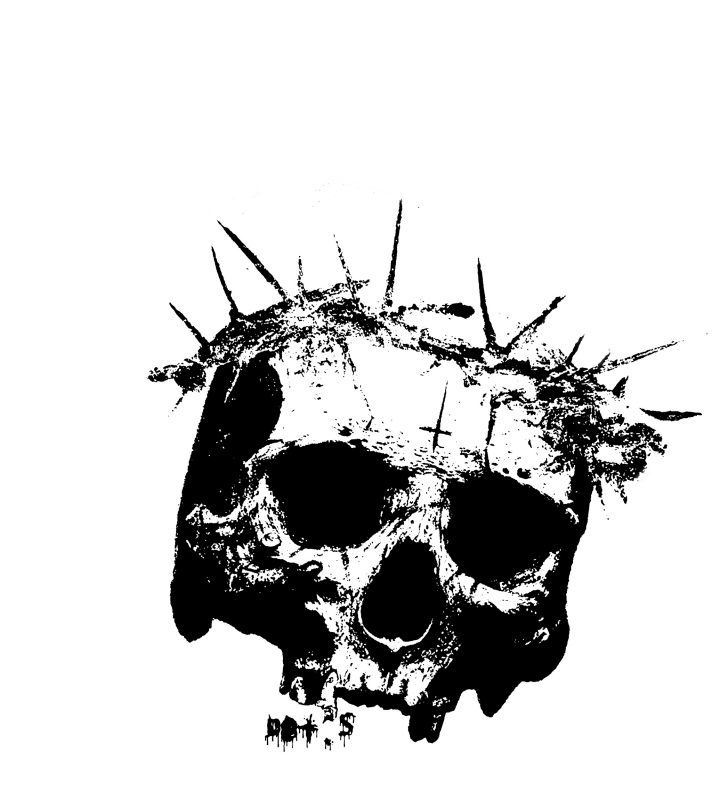
\includegraphics[width=\linewidth,keepaspectratio=true]{cunning/CunningHeader}
    \end{center}
    \newpage
}


\renewcommand{\yggCunningText}{%

    \mybold{Cunning} is the catch-all term for the rituals, divination, sacrifices, and voodoo performed during Downtime.  Your abilities as one of the cunning folk are measured by \mybold{Cunning Pips} obtained through the Mystic Virtues of \mypg{Mombo and Cunning Folk}{mystic-virtue-cunning-folk}, and through \mypg{Advancement}{advancement}.

    Cunning Pips can be spent during the \mybold{Production Step} of \mypg{Downtime}{downtime}. Any Cunning Pips you don't spend during the Production Step are lost at the end of the step.

    Cunning also has a cost in coin representing the bribing of officials, purchase of various legal and illegal materials, rental of space to perform the magic, etc. The total cost to perform Cunning depends on the total number of Cunning Pips you spend: the first 5 pips will cost you 100 \FE \myital{each}; the next 5 pips cost you 100 \AG each; and every pip after that will cost you 100 \AU. For example, if you spend 12 Cunning pips, the total will be 500 \FE plus 500 \AG plus 200 \AU. 

    \mytable{Y Y} {
        \thead{\# Pips} & \thead{Coin per Pip} \\
    } {
        1-5 & 100\FE \\
        6-10 & 100\AG \\
        11+ & 100\AU
    }



Occultism and the creation of Marvels must be performed on \mybold{Unhallowed Earth}. You can either make Unhallowed Earth yourself for a single Cunning Pip (see the occult ritual below), or make use of a \mypg{Locus}{gear-services-loci} if one exists in the Settlement (this can be a Side Story all its own if the Arbiter chooses to do so!).

\cbreak

\myimage{cunning/Cunning1}


  \newpage
  %%%%%%%%%%%%%%%%%%%%%%%%%%%%%%%%%%%%%%%%%%%%
%%% Marvels
%%%%%%%%%%%%%%%%%%%%%%%%%%%%%%%%%%%%%%%%%%%%

\mysection{Marvels}{cunning-marvels}

\flavor{"Terrific, a Six Demon Bag. Sensational. What's in it Egg?" \\~"Wind! Fire!  All that kind of thing!"  \\~ \Tilde Jack Burton and Egg Shen \\~ Big Trouble in Little China}

    \mytable{Y Y} {
        \thead{\# Pips} & \thead{Coin per Pip} \\
    } {
        1-5 & 100\FE \\
        6-10 & 100\AG \\
        11+ & 100\AU
    }


\begin{center}
\myredbold{Marvels take Weeks to create}
\end{center}



Ornately carved scrimshaw; shruken, leathery heads; straw stuffed poppets and crystal balls.  Marvels are magical baubles, knickknacks, and trinkets imbued with drops of \mylink{the Void}{the-void}, bound to \mylink{the Dream}{the-dream} with a Mystic's Cunning.


Marvels must be created from materials that are special or remarkable in some way. For example:

\mybullet {
  \item A carved branch of a tree that only grows in the cold stone ruins of Carcosa;
  \item 3 jeweled eggs stolen from a Roc's nest when the Eye of Tartarus is full;
  \item The carved fingerbones of St. Sacrastine, which reside in the sacristy of the Temple of Gomorrah in Lankhmar;
  \item etc.
}

Final OK is up to the Arbiter. Once you have the item, you spend your Cunning pips during \mylink{Downtime}{downtime} to imbue it with a few drops of the Void. Each Marvel must have a \mylink{Witch Mark}{occultism-witch-mark} on it for every unique power that it has (at the Arbiter's discretion).  The most common Marvels are listed below, but feel free to create your own.



\cbreak

\callout {
    If you're creating your own Marvel, tell the Arbiter what you want it to do, and she'll respond with the cost in Cunning Pips as well as any special ingredients it might require. The Arbiter gets the final OK. Additionally, Marvels follow the following rules:

    \mybullet {
      \item They cannot be used to deal direct damage, or be an item that causes damage directly (knives, swords, etc);
      \item They cannot be used to create a \DCUP or \DCDOWN effect;
      \item They cannot duplicate the effect of any \mylink{Arcana}{arcana} or \mylink{Vulgate}{vulgate}; and
      \item They cannot provide more than +4 to a specific \RO or \RB attempt.
    }
}



\mysubsection{Common Marvels}{cunning-common-marvels}

\MARVELS[
  Name=Adder's Tongue,
  Link=marvels-adders-tongue,
  Pips=2+
]

A single necklace of pierced adders' tongues, dipped in gold. Each tongue requires 2 Cunning to enchant, and allows the wearer to read and write one  \mylink{Language}{civilization-languages}. The Adventurer decides which languages the tongue(s) are attuned to when they put on the necklace.


\MARVELS[
  Name=Bezoar,
  Link=marvels-bezoar,
  Pips=4+
]

Super-gross mass of stuff, usually shoved into a pocket or carried in a small bag. The Bezoar provides +1 (4 Cunning Pips), +2 (8 Cunning Pips), +3 (12 Cunning Pips), or +4 (16 Cunning Pips) to Saves vs. Toxins.

\MARVELS[
  Name=Bone Abacus,
  Link=marvels-bone-abacus,
  Pips=2+
]

Adventurer's who use the Bone Abacus to do their calculations receive a +1 (2 Cunning Pips), +2 (4 Cunning Pips), +3 (6 Cunning Pips), or +4 (8 Cunning Pips) to their \mylink{Skill: Math}{skill-math} tries.

\MARVELS[
  Name=Bracelets of Muleskin,
  Link=marvels-bracelets-muleskin,
  Pips=1+
]

Hairy grey wristbands of muleskin, etched with runes.  The Adventurer increases their possible \mylink{Burden}{gear-burden} by +1 for each Cunning Pip spent.


\MARVELS[
  Name=Cat's Paw,
  Link=marvels-cats-paw,
  Pips=2+
]

A feline paw, typically worn hanging from a string or chain around the neck. If the wearer chooses, they can "burn" one of the "lives" that resides inside the Cat's Paw, allowing them to immediately succeed on a \DEATH try without rolling. The wearer must choose to use the power of the Cat's Paw \myital{instead of} rolling their \DEATH. The Cat's Paw contains 1 "life" in it for every 2 Cunning Pips spent.

There is a catch. If you choose to use a Cat's Paw when there are no lives left inside of it, you \myital{immediately} perish. If a Cat's Paw is found as part of a treasure haul, the Arbiter should roll a d10 in secret to determine how many lives are left (rolling a 10 means the Cat's Paw has no power inside of it, and will kill anyone foolish enough to try to use it). The \mylink{Third Eye Charm}{vulgate-charms}; the Virtue of Feyness (\mylink{Mystic}{adv-mystic-feyness} or \mylink{Spriggan}{adv-spriggan-feyness}); or the Spriggan Virtue of \mylink{The Eye}{adv-spriggan-the-eye} can tell you how many lives remain inside the paw.


\MARVELS[
  Name=Cornicello,
  Link=marvels-cornicello,
  Pips=4+
]

A twisted, horn-shaped charm made from bone, terracotta, or red coral and worn as a necklace or hung from a bracelet. The Cornicello provides +1 (4 Cunning Pips), +2 (8 Cunning Pips), +3 (12 Cunning Pips), or +4 (16 Cunning Pips) to Saves vs. Doom.

\cbreak

\MARVELS[
  Name=Cornucopia,
  Link=marvels-cornucopia,
  Pips=4
]

The horn of plenty will produce enough food and water to feed the entire \mylink{Band}{roles-band} during a \mylink{Bivouac}{combat-resting-bivouac} (no one needs to roll a \mylink{Provisions}{gear-equipment} \UD).  You need to place the Cornucopia on a flat surface for it to work - but it can't be placed on the ground.

\MARVELS[
  Name=Fish Mask,
  Link=marvels-fish-mask,
  Pips=2
]

An iron mask vaguely resembling some sort of aquatic creature.  When worn, the Adventurer may breathe underwater as if they were breathing normal air (unfortunately, breathing normal air is the same as trying to breathe water).


\MARVELS[
  Name=Forbidden Fruit,
  Link=marvels-forbidden-fruit,
  Pips=8
]

You create the "perfect" fruit - a shiny and ripe apple; a thick pomegranate; a juicy orange; etc. If proferred to someone, the victim must Save vs. Hexes or be compelled to take a bite. Once a bite is taken from the fruit, its enchantment ends. \mylink{Toxins}{malignants-toxins} can be injected into the fruit via syringe, if desired.


\MARVELS[
  Name=Golden Ankh,
  Link=marvels-ankh,
  Pips=8
]

The Golden Ankh is usually fastened with a cord and worn as a necklace, but it can also be an earring, hung from a belt, etc. The Adventurer in possession of an Ankh only fails their \mylink{Death}{adventurer-kismet-death} try if they roll a 1 (instead of a 1 or a 2).

\MARVELS[
  Name=Hammerspace Bag,
  Link=marvels-hammerspace-bag,
  Pips=2+
]

A sack or satchel made of spidersilk, the \mybold{Hammerspace Bag} can store a few kg of insignificant items (Arbiter's discretion) and/or a number of significant items with a \mylink{Burden}{gear-burden} equal to the Cunning Pips spent. The objects are stored in \mylink{Hammerspace}{meta-hammerspace}. Whatever you're looking for is always at the top of the bag.  Turning the bag upside down and shaking it will cause everything to fall out.

\MARVELS[
  Name=Ivory Earnhorn,
  Link=marvels-ivory-earhorn,
  Pips=2+
]

When the ivory earhorn is held up to the ear, the Adventurer gains a +1 (2 Cunning Pips), +2 (4 Cunning Pips), +3 (6 Cunning Pips), or +4 (8 Cunning Pips) to their \mylink{Skill: Listen}{skill-listen} tries.


\MARVELS[
  Name=Lucky Horseshoe,
  Link=marvels-lucky-horseshoe,
  Pips=2+
]

A rusty horseshoe with a four-leaf clover embossed at the base, the Adventurer holding it receives a +1 (2 Cunning Pips), +2 (4 Cunning Pips), +3 (6 Cunning Pips), or +4 (8 Cunning Pips) to their \mylink{Skill: Travel}{skill-travel} tries.


\MARVELS[
  Name=Lucky Rabbit's Foot,
  Link=marvels-lucky-rabbits-foot,
  Pips=8
]

An usually large rabbit's foot with a silver cap on one end. Those in possession of a Lucky Rabbit's Foot only fail their \mylink{Injury}{adventurer-kismet-injury} try if they roll a 1 (instead of a 1 or a 2). You probably shouldn't show this to a Pooka, they get pretty upset ...


\MARVELS[
  Name=Magic Jar,
  Link=marvels-magic-jar,
  Pips=12
]

An enchanted oil lamp / jar of stoneware / palm-sized iron box / stoppered bottle / etc. marked with runes. By Concentrating for Minutes, a Mortal Adventurer in possession of the Magic Jar may remove their soul and seal it inside. The Adventurer may at any time remove the soul from the container and place it back "inside" themselves by again Concentrating for Minutes.

There's only room for one soul inside the Magic Jar. A Mortal Adventurer can only restore their own soul and no one else's.  Any time they remove or restore their soul from the Magic Jar, they must make an \INSANITY try. Adventurers who have had their souls removed take on the \mybold{Unhallowed} trait. If the Mortal is killed while their soul is inside of the Magic Jar, their body flashes immediately out of existence (as if they were Unseelie) and their soul becomes an \mylink{Unquiet Spirit}{monster-unquiet-spirit} (an Apparition, Spook, Phantom, or Ghost depending on how powerful they were in life. See the section on \mylink{Monsters}{monsters} for more info). This spirit is trapped inside of the Magic Jar, and will burst forth in a terrible anger as soon as the oil lamp is rubbed, stoneware is broken, or box is opened.

An \mylink{Unseelie}{the-inhabitants} may remove the soul stored in the Magic Jar and place it in themselves, removing their \mybold{Unhallowed} trait (and making them immune to \mylink{Curse the Unhallowed}{vulgate-sacrament-curse-the-unhallowed}, allowing them to enter \mylink{Hallowed Ground}{miracle-hallowed-ground}, etc.). If an Unseelie dies while possessed by a Mortal soul, it immediately departs to the Void and drags the soul with it for an eternity of torment.

Losing a Magic Jar with your soul in it is ... bad. Mystical creatures and demons often use souls as bargaining chips, trades, "ingredients", etc. and will pay a good price for a Mortal soul. 



\MARVELS[
  Name=Mermaid's Scale,
  Link=marvels-mermaids-scale,
  Pips=2+
]

The scale is from the area near the waist, and marred with black runes. When held, the Adventurer gains a +1 (2 Cunning Pips), +2 (4 Cunning Pips), +3 (6 Cunning Pips), or +4 (8 Cunning Pips) to their \mylink{Skill: Salt}{skill-salt} tries.

\newpage

\MARVELS[
  Name=Poppet,
  Link=marvels-poppet,
  Pips=1+
]

A little rag doll or sock puppet, the Poppet will absorb a number of \mylink{Secrets of the Mind}{arcana-wizardry-secrets-alignment} equal to the number of Cunning Pips spent in its creation. When the Poppet absorbs the last effect, it falls apart. The owner of the Poppet will know if a Secret is cast on them, and whether or not the Poppet absorbed its effect.

\MARVELS[
  Name=Scrying Vessel,
  Link=marvels-scrying-vessel,
  Pips=4
]

Orbuculums, magic mirrors, crystal balls, etc. - a necessary bit of equipment for those wishing to practice \mylink{Descrying}{occultism-descry}.

\MARVELS[
  Name=Seer's Pipe,
  Link=marvels-seers-pipe,
  Pips=2+
]

When smoked with \mylink{Pipeweed}{gear-narcotics-pipeweed}, the Adventurer receives a +1 (2 Cunning Pips), +2 (4 Cunning Pips), +3 (6 Cunning Pips), or +4 (8 Cunning Pips) to their \mylink{Skill: Lore}{skill-lore} tries (on top of the bonus for the Pipeweed).

\MARVELS[
  Name=Shrunken Head,
  Link=marvels-shrunken-head,
  Pips=8
]

Usually hung from the belt, an Adventurer in possession of a Shrunken Head only fails their \mylink{Insanity}{adventurer-kismet-insanity} try if they roll a 1 (instead of a 1 or a 2).



\MARVELS[
  Name=Silver Bolt,
  Link=marvels-silver-bolt,
  Pips=2
]

A holly-branch missile with a silver tip, the Silver Bolt deals +d4 damage against Unhallowed creatures, and +3d4 damage against \mylink{the Damned}{forgotten-fealty-damned}. 

\cbreak

\MARVELS[
  Name=Silver Monocle,
  Link=marvels-silver-monocle,
  Pips=2+
]

If any Adventurer firmly grips the Silver Monocle in their eyesocket, they receive a +1 (2 Cunning Pips), +2 (4 Cunning Pips), +3 (6 Cunning Pips), or +4 (8 Cunning Pips) to their \mylink{Skill: Eyeball}{skill-eyeball} tries.

 
\MARVELS[
  Name=Talisman,
  Link=marvels-talisman,
  Pips=4+
]

A parchment, small knife, flat disc, etc. inscribed with runes. The Talisman provides +1 (4 Cunning Pips), +2 (8 Cunning Pips), +3 (12 Cunning Pips), or +4 (16 Cunning Pips) to Saves vs. Hexes.


\MARVELS[
  Name=Voodoo Doll,
  Link=marvels-voodoo-doll,
  Pips=12
]

A cloth, wax, or wooden doll with a simple yet somehow gruesome visage. By holding the Voodoo doll in front of yourself and concentrating on one Close or Nearby Monster (or Ally) that is wounded, you inflict them with \mylink{Bleeding}{effect-bleeding} for as long as you \mylink{Concentrate}{time-concentration}. You must mumble constantly while Concentrating - not loud, but not a whisper either.

\MARVELS[
  Name=Witch Bottle,
  Link=marvels-witch-bottle,
  Pips=2
]

A greybeard or bellarmine made of stoneware, glazed with salt, and embossed with a bearded face. Used to store \mylink{Unhallowed Earth}{occultism-unhallowed-earth}.


\MARVELS[
  Name=Wolf Tooth,
  Link=marvels-wolf-tooth,
  Pips=2+
]

If pressed into an empty tooth socket, the Wolf Tooth binds to the gums and the Adventurer receives a +1 (2 Cunning Pips), +2 (4 Cunning Pips), +3 (6 Cunning Pips), or +4 (8 Cunning Pips) to their \mylink{Skill: Bushcraft}{skill-bushcraft} tries.



  \newpage
  %%%%%%%%%%%%%%%%%%%%%%%%%%%%%%%%%%%%%%%%%%%%
%%% OCCULTISM
%%%%%%%%%%%%%%%%%%%%%%%%%%%%%%%%%%%%%%%%%%%%

\newpage


\mysection{Occultism}{cunning-occultism}

\callout {
    \mytable{Y Y} {
        \thead{\# Pips} & \thead{Coin per Pip} \\
    } {
        1-5 & 100\FE \\
        6-10 & 100\AG \\
        11+ & 100\AU
    }
}


\myimage{cunning/CunningHound}

\OCCULT[
  Name=Barghest,
  Link=occultism-barghest,
  Pips=5,
  Time=Days
]

You summon a spectral black dog (a harbinger of death and misfortune) to torment a single person for 7 days.  You must whisper the birth name of the victim to the spectre; upon hearing it, the black dog will seek the victim out, traveling up to 100km a night to find them.  The barghest can only travel at night, and disappears at the first light of the rising sun.  The dog can see invisible or hidden creatures and will unerringly find the target provided they are within distance of the casting of the ritual.

Once found, the barghest will appear to the victim once every night.  The victim is permitted a \SAVE{Doom} when they see the Barghest; if they fail, they suffer the curse of the Barghest until it appears again at sunset.  Pooka are immune to Barghests, and if the victim is in a Band with the Pooka, they get two Saves.

If the victim fails their save, they suffer the following maledictions until the next sundown:

\callout {
\mybullet {
    \item They are unable to heal Grit.
    \item All \RO and \RB tests suffer a -4 penalty.
    \item All of their \mylink{Kismet}{adventurer-kismet} dice move \DCDOWN.
}}

The victim must be someone Hallowed and Mortal.  The ritual requires a dog (your familiar is fine) and an item belonging to the victim. No harm comes to the dog, but the spectral figure will resemble him or her if examined closely.

\OCCULT[
  Name=Bind Familiar,
  Link=occultism-bind-familiar,
  Pips=2,
  Time=Weeks
]

Your Familiar is an embodiment of the Void, bound to your soul.  They can be summoned and dismissed at will: they'll appear from a shadow (cat) or sewer grate (rat) or fly in through a window (raven), and they'll leave roughly the same way.  Familiars are Unhallowed, and grant you +1 Cunning Pip if they're with you when you practice Occultism.

Familiars can be sent on missions up to 10km away. By Concentrating, you can "link" your mind with theirs. In this state you can see what they see and hear what they hear.  While Concentrating, you can cast \mylink{Charms}{vulgate-charms} through your Familiar if you desire (should you know the Vulgate of Charms). While linked with your Familiar you can remember things your familiar remembers (so you could send them on a spying mission and later "remember" what they saw). While Familiars are themselves immune to \mylink{Secrets of the Mind}{arcana-wizardry-secrets-alignment}, if one of these Secrets is performed on them while you are linked you will need to \SAVE{Hexes} or be affected as if the Secret targeted you. 

You familiar can't read your mind. If they are Close or Nearby you can communicate verbally with them, though you cannot use words greater than 1 syllable.  You communicate in a language all your own that no one else understands.  They can follow simple instructions ("get the key on the desk", "chew through these ropes", "spy on that man") but not more complex ones ("pick the lock").  Your familiar can't talk. 

Familiars are \mylink{Monsters}{monsters} with a Power of "Weak" (3 \mylink{Health}{monster-health} per \HD). They have a number of \HD equal to your \LVL -1 i.e. at level 1, your Familiar is a 0 \HD creature with 1 Health; at level 2, a 1 \HD creature with 3 Health, etc. If they're ever attacked and they survive, they immediately \mylink{Adjourn}{forgotten-obliterated} (disappear) and won't return for the rest of the Session. If your Familiar dies, you immediately drop to 0 Grit and lose 1 Flesh permanently.


Finally, you can place a \mylink{Malison}{occultism-malison} on your Familiar; in the event of your death, the Familiar will stay with your body until someone attempts to disturb your corpse.  At that point, it will deliver the Curse etched upon its skin, and Adjourn for good.

When you summon your Familiar, roll below (or discuss with the Arbiter if you want to choose), or make something up.  You can only have 1 Familiar at a time.



\myhighlight{Familiars}{occultism-familiars}

  \mytable{Y Y}{
    \thead{d6} & \thead{Familiar}\\
  }{
    1 & Cat \\
    2 & Dog \\
    3 & Rat \\
    4 & Toad \\
    5 & Raven \\
    6 & Exotic (roll below) \\
  }  

\begin{center}
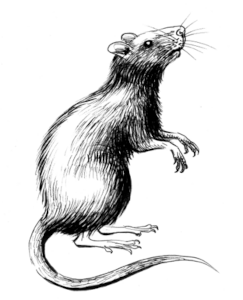
\includegraphics[scale=.2]{cunning/Rat}
\end{center}

  \mytable{l X}{
    \thead{d6} & \thead{Familiar}\\
  }{
    1 & The severed hands of a tomb robber  \\
    2 &  A floating piece of quartz \\
    3 & A 9-segmented colored cube that turns constantly  \\
    4 & A button-eyed doll made of rags and straw \\
    5 &  A tiny deformed homonculous resembling you \\
    6 & A hyper-intelligent slime \\
  }  



\OCCULT[
  Name=Damning,
  Link=occultism-damning,
  Pips=5,
  Time=Days
]

When you perform this ritual on a Mortal corpse no more than 7 days dead, you prevent them from departing \mylink{Limbo}{the-afterlife}.  The soul is trapped in Limbo permanently (though their soul can still be lead back to the Mortal plane through \mylink{Katabasis}{occultism-katabasis}).  The corpse is consumed when this ritual is performed.


\OCCULT[
  Name=Descry,
  Link=occultism-descry,
  Pips=See below,
  Time=Days
]

For each Cunning Pip you spend, you can see events transpiring 100km away (so 2 Pips, 200km; 3 Pips, 300km; etc.) by gazing into a silver bowl, censer, crystal ball, mirror, or other mystical item. This item must be a \mylink{Scrying Vessel}{marvels-scrying-vessel} (see \mylink{Marvels}{cunning-marvels} for more info).  You only need to describe what you want to see and it will appear, but the vision is misty and it's hard to make out details.  You can't see things that you might not normally be able to see, so if you said you wanted to "see the body of Sir Tremalane on the northern battlefield", and the body was buried, you might only see a grave.

The scrying doesn't have to only show events of the present; for each Cunning Pip you spend (apart from the Cunning Pips for seeing over great distances), you can see 1 century into the past. You'd have to have a rough idea of what you'd want to see - "show me the temples of Syrinx before they were cast down" would work, but "show me the secret entrance to the Caverns of Chaos" wouldn't.  The more detailed the description of what you want to see, the better you see it.

\example {
    Katarina wishes to see the location of a temple as it stood 200 years in the past, located somewhere in the jungle in the 100km surrounding the city. She must spend 3 Cunning Pips (2 for the years, 1 for the distance) to descry the location.
}

  \myimage{cunning/Occult_2}

\cbreak


\OCCULT[
  Name=Geas,
  Link=occultism-geas,
  Pips=10,
  Time=Days
]

A Geas is a command that compels the victim to perform a certain action, or fulfill a certain condition. The Geas could be long or difficult, like "find me the Needle of Obscurity in the Endless Haystacks" - or something easy, like "don't ever talk to me again." The victim must win a \RBTRY{\FOC}{\FOC} contest against you; if they fail, the Geas takes effect. From then on, any day that is not spent fulfilling the Geas will have one of the following effects (roll each day):


\callout {
\mynumlist {
  \item Inflicted with a \mylink{Greater Curse}{cunning-curses} (re-roll any duplicates);
  \item Inflicted with a \mylink{Disease}{vulgate-medicine-diseases} (roll on the Diseases table, re-roll any duplicates);
  \item Inflicted with a \mylink{Wound}{physical-wound} (roll on the Wounds table as if the target had been brought to 0 Flesh);
  \item All facets of \mylink{Personality}{adventurer-personality} move \DCDOWN;
  \item Inability to "heal" in any way - you gain absolutely no benefits from resting;
  \item Roll again - the result of the roll is inflicted on the target's loved one / parent / child / friend / etc. instead.  If the target loves nothing, the Arbiter gets to choose.
}
}

The effect lasts until sundown; provided the subject of the Geas is "back on track", the effect ends - otherwise, roll again.

The Geas must be doable, even if it is way above the means and possibility of the victim.  Should it become impossible (if the Endless Haystacks catch fire, for example), then the Geas is lifted.  Should you or the victim die, the Geas remains in effect, even if you are brought back from Limbo. This occultism cannot be performed on someone more than once in their lifetime.

On the upside, the Geas can empower its subject (at the Arbiter's discretion) to help them complete their task.  For example, if the Endless Haystacks are located in the fields outside of the cloud castle of the Giant King, the victim of the Geas might discover they have a handful of magic beans in their pocket that can help get them there.

The target of the Geas needs to be conscious and near you when you invoke the ritual.


\OCCULT[
  Name=Haunt,
  Link=occultism-haunt,
  Pips=5,
  Time=Days
]

You summon poltergeists to haunt an area up to 10km away. The area haunted has to be a distinct place (a graveyard, a house, etc.) no more than 100 square meters in size, and the haunting must be centered on a personal \mylink{Witch Mark}{occultism-witch-mark}. The poltergeists will cause chaos and mischief to any Mortals other than the invoker who enter their domain. They can neither talk nor directly harm anyone, but they will laugh unnervingly, appear as visible apparations, shake chains, throw things telekinetically about the room, etc. Meaningful rest (except a Breather) in a Haunted place is impossible, as is any ability or Arcana that requires Concentration. The grounds of the Haunting are considered \mylink{Unhallowed Earth}{occultism-unhallowed-earth}. The Haunting can only be ended by the removal of the Witch Mark (see description for methods of erasure).

\begin{center}
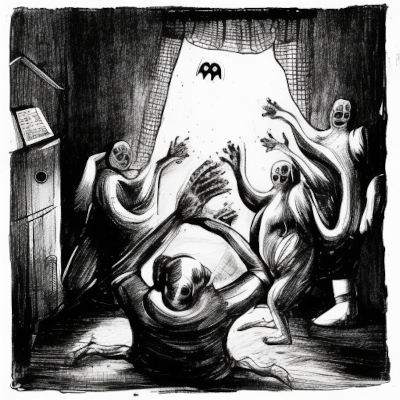
\includegraphics[scale=.45]{cunning/Poltergeist}
\end{center} 

\cbreak

  \myimage{cunning/Occult_3}

\OCCULT[
  Name=Hekaphage,
  Link=occultism-hekaphage,
  Pips=1+,
  Time=Days
]

\callout {
    For a Curse removed by a \mylink{Mundunugu}{gear-services}, multiply the costs by 5x (so 100\AG for a Lesser Curse and 500\AG for a Greater Curse).
}


You can destroy a curse by feeding it to a \mybold{Hekaphage}, an ethereal creature that eats Curses.  The number of pips required depends on the strength of the Curse:

\mybullet{
    \item a Lesser Curse requires 1 Cunning Pip
    \item a Greater Curse requires 5 Cunning Pips
}



\newpage


\OCCULT[
  Name=Katabasis,
  Link=occultism-katabasis,
  Pips=20,
  Time=Days
]

\summary {
    See the section on \mylink{the Afterlife}{the-afterlife} for more info about Limbo.
}

You open the door to \mylink{Limbo}{the-afterlife}, where the souls of the Hallowed dead must reside for 7 days before they rejoin the side of \TheAuthority. Mortals who pass through this door can attempt to bring a soul back to the land of the living.

The ritual must take place on \mylink{Unhallowed Earth}{occultism-unhallowed-earth}, in a room with a single door and no windows. By inhaling a special incense / partaking of a sacred mushroom / drinking a poisonous concoction / etc. up to 6 Mortals may pass through the door and enter the sorrowful plane of Limbo. The ritualist (you) must remain behind to keep the door open. You can keep the door open for as long as you \mylink{Concentrate}{time-concentration}; if your Concentration is broken, the door shuts, and those on the other side are lost.

Each Mortal who enters Limbo must carry a possession of the deceased: a sword, comb, lock of hair, etc. As long as they have this object in their possession, they have a rough idea of where the soul of the departed currently is. Additionally, they must bring two gold coins with them to pay the ferryman / conductor / guide / mayor / etc. who transports souls through Limbo, or use the coins to bribe ravens / make phonecalls / drop into wishing wells / etc.  The purpose of the coins seems to always vary, but anyone who walks through the door without these coins never returns. Finally, the Adventurers must carry a \mylink{Magic Jar}{marvels-magic-jar} (see \mylink{Marvels}{cunning-marvels}) through the doorway to transport the soul back home. A Magic Jar in Limbo attracts much attention ...

Once the soul is found, it must be placed into the Magic Jar to be transported across the threshold of Limbo. Manifold are the wonders of Limbo, and the soul may wish to remain rather than return to its humdrum life. It is better if a soul is coaxed within, rather than coerced. A Mortal can force a soul in Limbo into a Magic Jar against its will, but doing so consigns the vessel of the soul to permanent \mylink{Melancholy}{injury-insanity-madness}.

If a soul is successfully returned to the lands of the living, and their corpse is within the confines of the room, they may inhabit the body at no penalty (though an \INSANITY try is required).  If the corpse is absent, the Mortal will be reincarnated - the Player must move their Adventurer's Glory to the lowest number for their level (so if they were Level 7, they would move down to 32,000 Glory) and reroll their Adventurer.

Limbo will only permit a soul to be returned once. If a person should perish again, their souls become one of the \mylink{Forgotten}{the-forgotten}. Any Mortals that perish in Limbo are consumed in the same way.


\OCCULT[
  Name=Lichdom,
  Link=occultism-lichdom,
  Pips=20,
  Time=Months
]

This dangerous and depraved rite binds a Mortal's soul to a phylactery, allowing them to live on as a lich with life everlasting. Instead of the typical costs to perform a ritual, you must spend at least 25,000 \AU (higher costs at the Arbiter's discretion) for the necessary complex magical and chemical apparatus; bribes and dark gifts to creatures unholy creatures; hard-to-come-by components; etc. In addition to this exhorbitant sum, this rite requires:

\mybullet {
    \item a \mylink{Magic Jar}{marvels-magic-jar} (see \mylink{Marvels}{cunning-marvels}), which will become the Lich's phylactery;
    \item a dagger or knife marked with a \mybold{Bloodletting} rune (see \mylink{Sword Magic}{wonder-sword-magic}); and
    \item a Mortal vessel - that is, a human corpse - dead for less than 7 days
}

The ritual must take place in a room suitable for \mylink{Katabasis}{occultism-katabasis}. There, the deathly aspirant places their soul into the Magic Jar, stands in the doorway of Limbo, allows their jugular to be slit with the Bloodletting knife, and crosses the threshold with the Jar just as they expire.

\newpage

\myimage{cunning/Lichdom}

\cbreak

The Lich-to-be must bargain with the demons and devils of Limbo for life everlasting; their price should be high, and suitably depraved. Should the payment prove suitable, the Lich is permitted to return to the lands of the living carrying the Magic Jar with their soul inside.

The Magic Jar of this unholy creature is known as a \mybold{Phylactery}; so long as it remains intact, the Lich will live forever. If a Lich is slain, it will reform near their Phylactery at the next sunset. Liches have all of the powers, abilities, and memories they had in their Mortal form, and an endless amount of time to learn new things. In addition:

\callout{
\mybullet {
    \item The Lich ages one year for every 10 years that pass (very old liches tend to look cadaverous or skeletal);
    \item The Lich is immune to non-magical weapons, \mylink{Toxins}{malignants-toxins}, \mylink{Secrets of the Mind}{arcana-wizardry-secrets-alignment}, and \mylink{Secrets of Entropy}{arcana-wizardry-secrets-alignment}; and
    \item If the Lich knows any Secrets, they may write as many of them as they desire into their skulls (see \mylink{Sorcerer's Skull}{arcana-wizardry-skull} under \mylink{Wizardry}{arcana-wizardry}) - making them extremely potent Fetishes in their own right!
}}

Liches are \mybold{Unhallowed}. If their phylactery is destroyed or opened, they immediately disappear in a dazzling flash, their souls returned to Limbo for eternal torment. 

\newpage

\OCCULT[
  Name=Malison,
  Link=occultism-malison,
  Pips=2+,
  Time=Days
]

You place a \mylink{Curse}{cunning-curses} ...

\mylist {
  \item ... on a person within 1km; 
  \item ... on a \mylink{Marvel}{cunning-marvels};  
  \item ... on your \mylink{Familiar}{occultism-familiars}; or
  \item ... on a \mylink{Cursing Sigil}{inscription-sigil-cursing}
}

The cost varies:

\mybullet{
    \item a \myital{random} Lesser Curse requires 2 Cunning Pips.
    \item a \myital{specific} Lesser Curse requires 6 Cunning Pips.
    \item a \myital{random} Greater Curse requires 10 Cunning Pips.
    \item a \myital{specific} Greater Curse requires 14 Cunning Pips.

}

You can break any of your own curses at will. Malisons will survive your death.  \mylink{Pooka}{species-pooka} are immune to your Malison.

\cbreak

\OCCULT[
  Name=Unhallowed Earth,
  Link=occultism-unhallowed-earth,
  Pips=2,
  Time=Days
]

Through the Occultism of Unhallowed Earth, you desecrate a handful of earth and imbue it with the chaos energy of the Void. Unhallowed Earth must be stored in a \mylink{Witch Bottle}{marvels-witch-bottle} until you are ready to use it. When poured on the ground, the soil desecrates an area 10 meters in radius. If the ground that is desecreated is \mylink{Hallowed Ground}{miracle-hallowed-ground}, the blessing is removed. Otherwise no Mortal or Hallowed creature may enter Unhallowed Earth unless they are invited by the Mystic who created it or they bear their \mylink{Witch Mark}{occultism-witch-mark}; and no \mylink{Sacraments}{vulgate-sacraments} may be performed on its soil.



\OCCULT[
  Name=Witch Mark,
  Link=occultism-witch-mark,
  Pips=1,
  Time=Days
]

A smear of the Void is placed on a person or thing, only visible to the Unseelie and to Mortals using the Charm of the \mylink{Third Eye}{vulgate-charms} (see the \mylink{Vulgate of Charms}{vulgate-charms}). Your Witch Mark is unique, like a fingerprint or calling card. Unless you've seen a particular Witch Mark before, a \mylink{Skill: Lore}{skill-lore} try is required to determine the owner of the Witch Mark. Mortal creatures marked with a Witch Mark are \mybold{Unhallowed} for either 7 days or until the end of the Session (whichever comes first); otherwise, a Witch Mark can only be removed by the witch who placed it there, or by sprinkling the symbol with a pinch of \mylink{Hallowed Ground}{miracle-hallowed-ground}.

  \newpage
  \end{multicols*}

\mysection{Curses}{cunning-curses}

Curses can be broken by the cunning folk who have placed them; by employing the services of a \mylink{Mundunugu}{gear-services}; by the miracle of \mylink{Sin Eating}{miracle-sin-eating}; or by feeding them to a \mylink{Hekaphage}{occultism-hekaphage} (provided you know the ritual, of course). \mylink{Pooka}{species-pooka} are immune to curses. 

These are just a few ideas to get you started; the devious Arbiter is encouraged to concoct her own!


  \mysubsection{Lesser Curses}{table-lesser-curses}

  \mytable{l X} {  
  } {
    1 & All of your hair immediately falls off in a pile on the floor, and won't grow back. \\
    2 & You can't enter a house or cross a threshold without the permission of someone already inside. \\
    3 & You can't cross running water (even over a bridge) unless someone carries you. \\
    4 & You sprout thick, white hair from the palms of your hands and your ears.  Close observation shows very tiny translucent crabs that make their home in the strands.  No one wants to shake your hand, but cats love licking up the crabs. \\
    5 & You are unable to speak your own name \\
    6 & The Arbiter gives you a new name.  Everyone (except you) thinks this is your real name, and you can't change their mind. \\
    7 & You become \mylink{Unseelie}{the-inhabitants} (and therefore \mylink{Unhallowed}{effect-unhallowed}). \\
    8 & Like a \mylink{Spriggan}{species-spriggan}, you can't hold anything made of Iron.  If you do, you take 1 point of damage directly to Flesh every Moment. \\
    9 & A small imp appears on your shoulder. The imp is played by the Arbiter, and causes no end of mischief.  You can slap, step on, stab, etc. the imp, who immediately disappears with a pop - but returns in Minutes.  Angry. \\
    10 & You fall into deep slumber when you hear music. You can only be woken by being shaken / slapped awake. \\
    11 & Everything you say is believed to be a lie \\
    12 & You can only speak in rhymes. \\
}



  \mysubsection{Greater Curses}{table-greater-curses}


  \mytable{l X} {  
  } {

    1 & Leaden. Your limbs become leaden and weighty, and now have a \mylink{Burden}{gear-burden} of 4. \\
    2 & Unhanded. Roll a d6. 1-3 Your non-dominant hand disappears. 4-5 Your dominant hand disappears. 6 They both disappear. \\
    3 & Poverty. You are unable to hold coins of any sort.  Handing you any coins makes the coins disappear, permanently. \\
    4 & Dyslexia. You cannot read written words (including from a \mylink{Grimoire}{grimoires}). \\
    5 & Blindness. Your eyes disappear from your face. You are \mylink{Blinded}{effect-blinded}. \\
    6 & Deafness. Your ears disappear from your head. You are \mylink{Deafened}{effect-deafened}. \\
    7 & Triskaidekaphobia. For any die you roll, if you roll a 13, treat it as a natural 1. \\
    8 & Vampiric. The sun burns and blisters your skin, doing 1 Flesh damage for every Moment in direct sunlight. You cannot regain Grit unless you first drink the blood of a living thing (not enough to kill them, about a cupful). \\
    9 & Ghastly. You can't add the result of a \mylink{Personality}{adventurer-personality} try to any \RO or \RB attempt. \\
    10 & Excommunicated. You suffer from \mylink{Anathema}{effect-anathema}. \\
    11 & Noisy. When you are sneaking around, you have an uncontrollable urge to sing "Here Comes a Sneaky Boy!" at top volume (regardless of gender).  Stealth is impossible. \\
    12 & Voiceless. Your vocal cords are paralyzed and you cannot speak. \\
}

\begin{multicols*}{2}


}%end
